\documentclass{article}
\usepackage{graphicx} % Required for inserting images
\usepackage[polish]{babel}
\usepackage{hyperref}
\usepackage[T1]{fontenc}

\title{Eliminacja Gaussa}
\author{Filip Jędrzejewski}
\date{24 Grudnia 2023}

\begin{document}

\maketitle

\section{Wstęp}

\subsection{Cel zadania}

Celem zadania było zaprojektowanie i zaimplementowanie równoległego algorytmu eliminacji Gaussa.

\subsection{Informacje o programie}

Program został w całości napisany w języku \texttt{c++}. Dane wejściowe do programu są wczytywane z pliku \texttt{.txt}, natomiast wynik wypisywany jest w terminalu.

\subsection{Zaimplementowane funkcjonalności}

W programie zaimplementowano następujące funkcjonalności:
\begin{itemize}
    \item Transponowanie danej macierzy
    \item Współbieżny algorytm eliminacji Gaussa doproawdzający daną macierz do postaci górnej trójkątnej
    \item Iteracyjny algorytm eliminacji Gaussa
    \item Obliczanie wyznacznika danej macierzy z definicji
    \item Obliczanie wyznacznika danej macierzy korzystając z równoległej eliminacji Gaussa
    \item Rozwiązywanie układu równań liniowych danego w postaci macierzowej
\end{itemize}

\section{Opis teoretyczny}

W celu rozwiązania zadania zdefiniowano następujące operacje:
\begin{itemize}
    \item $A_{i,j}$ - wyznaczenie mnożnika dla wiersza $i$, by odjąć go od wiersza $j$.
    \item $B_{i,k,j}$ - przemnożenie elementu $k$ z wiersza $i$, przez mnożnik dla wiersza $j$.
    \item $C_{i,k,j}$ - odjęcie elementu $k$ z wiersza $i$ od elementu $k$ z wiersza $j$.
\end{itemize}

Na podstawie tej listy operacji stworzono grafy Diekerta dla współbieżnego algorytmu eliminacji Gaussa dla macierzy o rozmiarach: 2x2, 3x2, 3x3, 4x3 oraz 4x4, by znaleźć zależności, które by pozwoliły na uogólnienie zależności między poszczególnymi operacjami dla dowolnych rozmiarów macierzy.


\begin{figure}[htb]
\centering
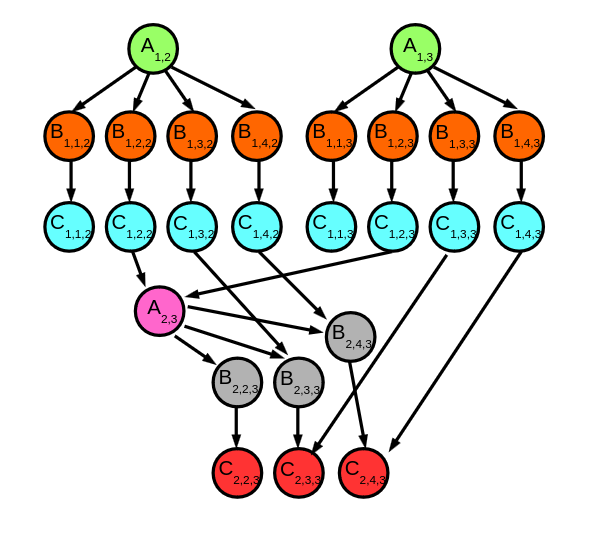
\includegraphics[width=10cm]{graf.png}
\caption{Przykładowy graf Diekerta dla macierzy 4x3}
\end{figure}


\section{Implementacja}

\subsection{Lista klas}

W programie stworzono następujące klasy:

\begin{enumerate}
    \item \texttt{InputParser} - klasa wykorzystywana do tworzenia obiektu macierzy (\texttt{Matrix}) z odczytanego pliku \texttt{.txt}.
    \item \texttt{Matrix} - klasa reprezentująca macierz, przechowująca ją i udostępniająca metody do jej obsługi.
    \item \texttt{Gauss} - klasa zawierająca metody do eliminacji Gaussa sposobem iteracyjnym lub współbieżnym oraz do rozwiązywania układów równań liniowych.
\end{enumerate}

\subsection{Opisy plików}

\subsubsection{./src/main.cpp}

Główny plik zawierający funkcję \texttt{int main()}m która otwiera plik z danymi wejściowymi, przekazuje je do obiektu klasy \texttt{InputParser}, uruchamia eliminację Gaussa, wyświetla otrzymaną macierz oraz rozwiązuje układ równań.

\subsubsection{./src/HeaderFiles/constants.h oraz interfaces.h}

Pliki nagłówkowe zawierające stałe oraz definicje zaimplementowanych klas.

\subsubsection{./src/InputLogic/InputParser.cpp}

Plik zawierający implementację klasy \texttt{InputParser} zdefiniowanej jako:

\begin{verbatim}
    class InputParser{
        private:
            int nx;
            int ny;
            Matrix* matrix;
        public:
            InputParser();
            ~InputParser();
            void createNewMatrix(int x, int y);
            void setRow(int i, std::string line);
            Matrix* getMatrix();
    };
\end{verbatim}

\subsubsection{./src/Matrix/Matrix.cpp}

Plik zawierający implementację klasy \texttt{Matrix} zdefiniowanej jako:

\begin{verbatim}
    class Matrix{
        private:
            int nx;
            int ny;
            float** tab;
            Matrix* getMatrixWithout(int ii, int ij);
        public:
            Matrix();
            Matrix(int nx, int ny);
            ~Matrix();
            void setValue(int i, int j, float value);
            void subtractRowsWithMultiplicator(int i1, int i2, float value);
            void multiplicateRow(int i, float value);
            int getSizeX();
            int getSizeY();
            float getValue(int i, int j);
            Matrix* getTransposedMatrix();
            Matrix* addColumns(Matrix* v);
            Matrix* popLastColumn();
            void show(std::string description);
            float getDet(char method);  //g - Gauss OR d - definition
    };
\end{verbatim}

Metoda \texttt{Matrix* getMatrixWithout(int ii, int ij)} zwraca obiekt macierzy powstałej po usunięciu wiersza \texttt{ii} oraz kolumny \texttt{ij}.

Metoda \texttt{Matrix* popLastColumn()} zwraca macierz będącą ostatnią kolumną oraz usuwa ostatnią kolumnę z macierzy początkowej.

Metoda \texttt{float getDet(char method)} zwraca wartość wyznacznika macierzy. Argument \texttt{char method} służy do określenia, z której metody funkcja ma skorzystać: \texttt{'g'} - metoda wykorzystująca współbieżny algorytm eliminacji Gaussa, \texttt{'d'} - metoda obliczająca wyznacznik korzystając z definicji.

\subsubsection{./src/Matrix/Gauss.cpp}

Plik zawierający implementację klasy \texttt{Gauss} zdefiniowanej jako:

\begin{verbatim}
    class Gauss{
        private:
            bool merged = false;
            Matrix* m;
            Matrix* v;
        public:
            Gauss();
            Gauss(Matrix* matrix);
            Gauss(Matrix* matrix, Matrix* vector);
            ~Gauss();
            void classicElimination();
            void threadElimination();
            void toIdentityMatrix();
            Matrix* getMatrix();
            Matrix* getVector();
    };
\end{verbatim}

Konstruktor \texttt{Gauss(Matrix* matrix, Matrix* vector)} łączy daną macierz i wektor w jedną macierz (dodaje do macierzy kolumnę zawierającą wektor).

Metoda \texttt{void classicElimination()} wykonuje eliminację Gaussa metodą iteracyjną.

Metoda \texttt{void threadElimination()} wykonuje równoległą eliminację Gaussa.

Metoda \texttt{void toIdentityMatrix()} rozwiązuje układ równań liniowych dany w postaci macierzowej (do klasy należy przekazać macierz współczynników oraz wektor wyrazów wolnych).

Metody \texttt{Matrix* getMatrix()} oraz \texttt{Matrix* getVector()} zwracają macierz i wektor, a w przypadku, gdy zostały one połączone w konstruktorze, wtedy również je rozdziela.



\section{Dane wejściowe}

Dane wejściowe do programu powinny być podane w pliku \texttt{./data/inputData.txt} w postaci:

\begin{verbatim}
    rozmiar macierzy
    macierz
    wektor w postaci transponowanej
\end{verbatim}

Przykładowa zawartość pliku \texttt{./data/inputData.txt}:

\begin{verbatim}
    3
    2.0 1.0 3.0
    4.0 3.0 8.0
    6.0 5.0 16.0
    6.0 15.0 27.0
\end{verbatim}

\subsection{Uwaga}
Program nie uwzględnia ewentualnej konieczności zamiany miejscami wierszy.



\section{Wyjście programu}

Program wypisuje dane wyjściowe w terminalu. W obecnej konfiguracji pliku \texttt{./src/main.cpp} wyjście programu wygląda następująco:

\begin{verbatim}
    macierz odczytana z pliku wejściowego
    wektor odczytany z pliku wejsciowego
    transponowany wektor
    macierz po równoległej eliminacji Gaussa
    wektor po równoległej eliminacji Gaussa
    macierz jednostkowa (otrzymana podczas rozwiązywania układu równań)
    wektor będący rozwiązaniem układu równań
\end{verbatim}

Dane zwrócone przez program dla przykładowych danych podanych w poprzedniej sekcji:

\begin{verbatim}
    Input matrix:
    | 2.00  1.00    3.00    |
    | 4.00  3.00    8.00    |
    | 6.00  5.00    16.00   |

    Input vector:
    | 6.00  15.00   27.00   |

    Transposed vector:
    | 6.00  |
    | 15.00 |
    | 27.00 |

    Matrix after elimination:
    | 2.00  1.00    3.00    |
    | 0.00  1.00    2.00    |
    | 0.00  0.00    3.00    |

    Vector after elimination:
    | 6.00  |
    | 3.00  |
    | 3.00  |

    Indentity matrix:
    | 1.00  0.00    0.00    |
    | 0.00  1.00    0.00    |
    | 0.00  0.00    1.00    |

    Vector:
    | 1.00  |
    | 1.00  |
    | 1.00  |
\end{verbatim}



























\end{document}